% ============================================================================
\section{Calibración de los parámetros}\label{sec:calibracion}
% ============================================================================

Esta sección aplica el procedimiento de la sección~\ref{sec:ofat} a las cinco
metaheurísticas. Para cada una hay una tabla (una fila por etapa, con el RPD medio de cada
valor probado) y una figura con los mismos datos, en la que la línea discontinua marca el
resultado de la búsqueda local sola: es la referencia que una metaheurística tiene que
mejorar para justificar sus 5 segundos. Todas las cifras son RPD medios sobre las 18
ejecuciones de cada configuración en las 6 instancias de calibración.

\begin{idea}[Sobre las cifras de esta sección]
Las tablas y figuras se generan automáticamente a partir de los ficheros de la carpeta
\cod{experimentos/}; los comentarios del texto se refieren a la ejecución de referencia con la
que se ha escrito la memoria. Si se repite la calibración en otro ordenador
(sección~\ref{sec:uso}), las tablas se actualizan solas al volver a ejecutar
\cod{generar\_tablas.py} y compilar, pero conviene releer los comentarios: las cifras
cambiarán algo y, en los parámetros poco sensibles, puede cambiar el valor elegido.
\end{idea}

% ----------------------------------------------------------------------------
\subsection{Temple Simulado}\label{sec:cal-temple}

\begin{table}[H]
\centering
\caption{Calibración de Temple Simulado. Cada fila es una etapa: RPD medio (\%) sobre las 18 ejecuciones (6 instancias $\times$ 3 semillas) de cada valor probado, con los demás parámetros fijos. En negrita, el mejor.}
\label{tab:cal-temple}
\small
\begin{tabular}{@{}cl>{\raggedright\arraybackslash}p{10.4cm}c@{}}
\toprule
Etapa & Parámetro & Valor probado $\rightarrow$ RPD medio & Elegido \\ \midrule
1 & \texttt{k} & 1\,$\rightarrow$\,6.451;\quad 2\,$\rightarrow$\,\textbf{4.597};\quad 3\,$\rightarrow$\,4.748;\quad 5\,$\rightarrow$\,5.611 & 2 \\
2 & \texttt{lrc} & 1\,$\rightarrow$\,4.766;\quad 2\,$\rightarrow$\,\textbf{4.597};\quad 3\,$\rightarrow$\,4.598;\quad 5\,$\rightarrow$\,4.605 & 2 \\
3 & \texttt{p0} & 0.02\,$\rightarrow$\,4.477;\quad 0.1\,$\rightarrow$\,\textbf{4.477};\quad 0.3\,$\rightarrow$\,4.496;\quad 0.5\,$\rightarrow$\,4.597 & 0.1 \\
4 & \texttt{alfa} & 0.9\,$\rightarrow$\,4.559;\quad 0.95\,$\rightarrow$\,4.477;\quad 0.99\,$\rightarrow$\,\textbf{4.127} & 0.99 \\
5 & \texttt{L} & 200\,$\rightarrow$\,4.935;\quad 1000\,$\rightarrow$\,\textbf{4.127};\quad 5000\,$\rightarrow$\,6.557 & 1000 \\
\bottomrule
\end{tabular}
\end{table}

\begin{figure}[H]\centering
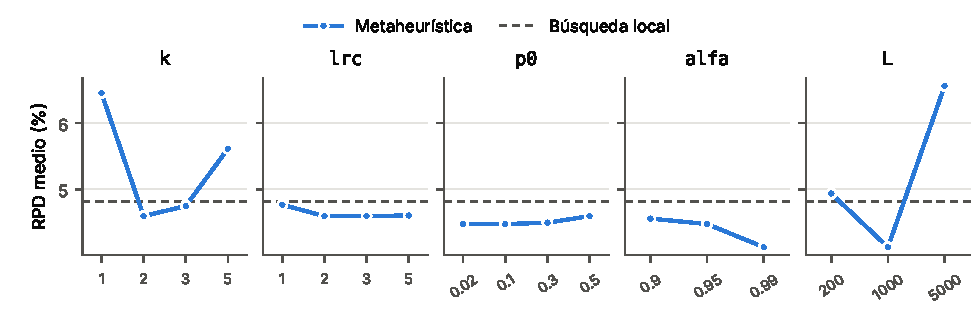
\includegraphics[width=\textwidth]{figuras/cal_temple.pdf}
\caption{Temple Simulado: RPD medio según el valor de cada parámetro.}
\end{figure}

\begin{itemize}
  \item \textbf{\cod{k} (tamaño de la vecindad): parámetro crítico.} Con $k=1$ el resultado
        (6.45) es prácticamente el del constructivo: al quitar una sola columna, la
        reparación voraz casi siempre vuelve a una solución equivalente y el temple no
        consigue moverse. Con $k=5$ (5.61) cada vecina es demasiado distinta y demasiado
        cara: se generan 138\,000 vecinas en lugar de 420\,000 y casi todas empeoran mucho.
        El mejor es $k=2$.
  \item \textbf{\cod{lrc}: basta con que no sea 1.} Con reparación determinista (1) el
        resultado es peor (4.77); entre 2, 3 y 5 la diferencia es de milésimas, es decir,
        un empate. Se conserva 2.
  \item \textbf{\cod{p0}: poco sensible.} De 0.02 a 0.3 no hay diferencias apreciables; 0.5
        es algo peor. Empezar muy caliente solo gasta tiempo aceptando empeoramientos. Se
        elige 0.1.
  \item \textbf{\cod{alfa} y \cod{L}: lo decisivo es la velocidad de enfriamiento.} Con
        $L=1000$ se recorren unas 420 temperaturas en los 5 segundos. Con $\alpha=0.99$ la
        temperatura final es $0.99^{420}\approx 0.015$ veces la inicial: un único
        enfriamiento lento que termina justo cuando se acaba el tiempo, y es lo mejor
        (4.13). Con $\alpha=0.95$ o $0.90$ el sistema se congela mucho antes y el resto del
        tiempo se va en recalentamientos (4.48 y 4.56). El caso $L=5000$ es muy instructivo:
        solo hay unas 100 temperaturas, la final es $0.99^{100}\approx 0.37$ veces la
        inicial, el sistema \emph{nunca llega a enfriarse} y el resultado (6.56) es el de la
        solución inicial: en 5 segundos no la mejora ni una vez. Con $L=200$ ocurre lo
        contrario: se enfría en un segundo y recalienta varias veces (4.94).
\end{itemize}

\textbf{Configuración elegida:} $k=2$, \cod{lrc}~$=2$, $p_0=0.1$, $\alpha=0.99$, $L=1000$. El
RPD pasa de 4.60 (base) a 4.13. La mejor solución se encuentra, de media, a los 4.1
segundos: el algoritmo sigue mejorando casi hasta el final, señal de que el enfriamiento
está bien ajustado al tiempo.

% ----------------------------------------------------------------------------
\subsection{Búsqueda Tabú}\label{sec:cal-tabu}

\begin{table}[H]
\centering
\caption{Calibración de Búsqueda Tabú. Cada fila es una etapa: RPD medio (\%) sobre las 18 ejecuciones (6 instancias $\times$ 3 semillas) de cada valor probado, con los demás parámetros fijos. En negrita, el mejor.}
\label{tab:cal-tabu}
\small
\begin{tabular}{@{}cl>{\raggedright\arraybackslash}p{10.4cm}c@{}}
\toprule
Etapa & Parámetro & Valor probado $\rightarrow$ RPD medio & Elegido \\ \midrule
1 & \texttt{tent} & 5\,$\rightarrow$\,4.215;\quad 10\,$\rightarrow$\,4.136;\quad 20\,$\rightarrow$\,\textbf{4.098};\quad 50\,$\rightarrow$\,4.280 & 20 \\
2 & \texttt{tsal} & 1\,$\rightarrow$\,\textbf{4.096};\quad 3\,$\rightarrow$\,4.098;\quad 5\,$\rightarrow$\,4.188;\quad 10\,$\rightarrow$\,4.196 & 1 \\
3 & \texttt{beta} & 0\,$\rightarrow$\,4.124;\quad 0.01\,$\rightarrow$\,\textbf{4.096};\quad 0.05\,$\rightarrow$\,4.323;\quad 0.2\,$\rightarrow$\,4.513 & 0.01 \\
4 & \texttt{reinicio} & 500\,$\rightarrow$\,4.145;\quad 2000\,$\rightarrow$\,4.096;\quad $10^6$\,$\rightarrow$\,\textbf{4.095} & $10^6$ \\
\bottomrule
\end{tabular}
\end{table}

\begin{figure}[H]\centering
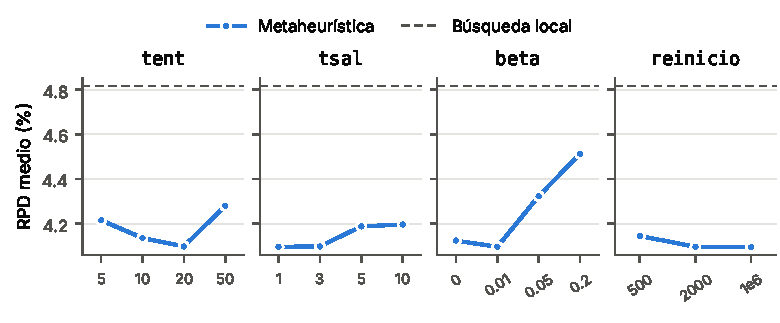
\includegraphics[width=0.85\textwidth]{figuras/cal_tabu.pdf}
\caption{Búsqueda Tabú: RPD medio según el valor de cada parámetro.}
\end{figure}

\begin{itemize}
  \item \textbf{\cod{tent} (duración tabú de entrada).} Curva en forma de U con el mínimo en
        20: con 5 la prohibición es demasiado corta (4.22) y con 50 se prohíben demasiadas
        columnas útiles (4.28).
  \item \textbf{\cod{tsal} (duración tabú de salida).} Como se había razonado en la
        sección~\ref{sec:tabu}, conviene que sea mucho más corta que la de entrada: 1 y 3
        empatan (4.10) y 5 o 10 son peores (4.19 y 4.20). Proteger durante mucho tiempo a
        las columnas recién llegadas bloquea la solución.
  \item \textbf{\cod{beta} (penalización por frecuencia).} Una penalización muy suave (0.01)
        es ligeramente mejor que ninguna (4.10 frente a 4.12, dentro del ruido), pero en
        cuanto crece empeora con claridad (4.32 y 4.51). Las frecuencias crecen sin límite
        a lo largo de la búsqueda, mientras que los valores de los movimientos son del orden
        de la unidad:
        con $\beta$ grande la penalización domina y la búsqueda deja de mirar el coste.
  \item \textbf{\cod{reinicio} (intensificación).} Volver a $s^\ast$ cada 500 iteraciones
        empeora un poco (4.15); cada 2000 o nunca da lo mismo (4.10). La intensificación por
        reinicio no aporta nada aquí.
\end{itemize}

\textbf{Configuración elegida:} \cod{tent}~$=20$, \cod{tsal}~$=1$, $\beta=0.01$, sin
reinicios. El RPD pasa de 4.14 a 4.10. \textbf{La búsqueda tabú es muy poco sensible a sus
parámetros}: entre la mejor y la peor configuración probada hay cuatro décimas. La mejor
solución aparece pronto (a los 1.6 segundos de media) y después la búsqueda se estanca, lo
que indica que su limitación no está en los parámetros sino en los movimientos.

% ----------------------------------------------------------------------------
\subsection{GRASP}\label{sec:cal-grasp}

\begin{table}[H]
\centering
\caption{Calibración de GRASP. Cada fila es una etapa: RPD medio (\%) sobre las 18 ejecuciones (6 instancias $\times$ 3 semillas) de cada valor probado, con los demás parámetros fijos. En negrita, el mejor.}
\label{tab:cal-grasp}
\small
\begin{tabular}{@{}cl>{\raggedright\arraybackslash}p{10.4cm}c@{}}
\toprule
Etapa & Parámetro & Valor probado $\rightarrow$ RPD medio & Elegido \\ \midrule
1 & \texttt{lrc} & 2\,$\rightarrow$\,4.149;\quad 3\,$\rightarrow$\,3.952;\quad 5\,$\rightarrow$\,3.729;\quad 10\,$\rightarrow$\,\textbf{3.533} & 10 \\
2 & \texttt{lamf} & 1.0\,$\rightarrow$\,4.322;\quad 0.8\,$\rightarrow$\,3.636;\quad 0.5\,$\rightarrow$\,3.533;\quad 0.2\,$\rightarrow$\,\textbf{3.519} & 0.2 \\
3 & \texttt{elite} & 5\,$\rightarrow$\,\textbf{3.441};\quad 10\,$\rightarrow$\,3.519;\quad 20\,$\rightarrow$\,3.726 & 5 \\
4 & \texttt{grent} & 2\,$\rightarrow$\,4.407;\quad 3\,$\rightarrow$\,\textbf{3.441} & 3 \\
\bottomrule
\end{tabular}
\end{table}

\begin{figure}[H]\centering
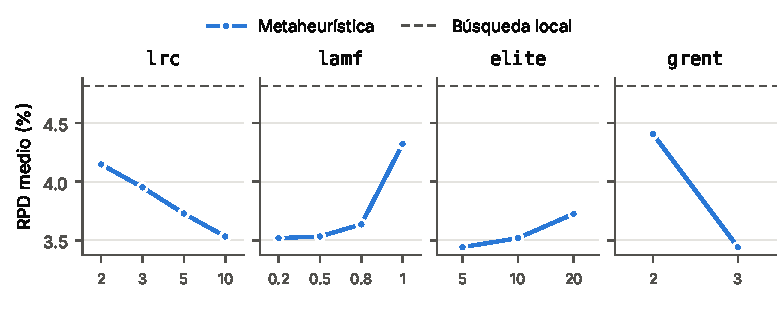
\includegraphics[width=0.85\textwidth]{figuras/cal_grasp.pdf}
\caption{GRASP: RPD medio según el valor de cada parámetro.}
\end{figure}

\begin{itemize}
  \item \textbf{\cod{lrc}.} El resultado mejora de forma continua al aumentar la lista: 4.15
        con 2 y 3.53 con 10. Más azar en la construcción da soluciones iniciales más
        variadas, y la búsqueda local se encarga de la calidad. Como gana el valor más
        grande de la lista, es posible que uno mayor sea todavía mejor: es el primer
        candidato para la segunda vuelta opcional.
  \item \textbf{\cod{lamf} (memoria): el componente más importante.} Sin memoria
        ($\lambda_f=1$, GRASP básico) el RPD es 4.32; con memoria baja a 3.52--3.64. Guiar la
        construcción hacia las columnas que aparecen en las mejores soluciones encontradas
        vale ocho décimas: es, con diferencia, el mecanismo de memoria más rentable de los
        cinco algoritmos. Entre
        $\lambda_f=0.5$ y $0.2$ hay empate.
  \item \textbf{\cod{elite}.} Mejor pequeño: 3.44 con 5 soluciones y 3.73 con 20. Un élite
        grande incluye soluciones mediocres y diluye la información.
  \item \textbf{\cod{grent}.} Con dos entornos se hacen más iteraciones (unas 600 frente a
        450) pero el resultado es mucho peor (4.41 frente a 3.44). Conviene gastar el tiempo
        en la mejora (el entorno $\D3$) y no en construir más soluciones, lo que responde a
        la pregunta que planteaban los apuntes.
\end{itemize}

\textbf{Configuración elegida:} \cod{lrc}~$=10$, $\lambda_f=0.2$, \cod{elite}~$=5$,
\cod{grent}~$=3$. El RPD pasa de 3.95 a 3.44.

% ----------------------------------------------------------------------------
\subsection{Algoritmo Genético}\label{sec:cal-genetico}

\begin{table}[H]
\centering
\caption{Calibración de Algoritmo Genético. Cada fila es una etapa: RPD medio (\%) sobre las 18 ejecuciones (6 instancias $\times$ 3 semillas) de cada valor probado, con los demás parámetros fijos. En negrita, el mejor.}
\label{tab:cal-genetico}
\small
\begin{tabular}{@{}cl>{\raggedright\arraybackslash}p{10.4cm}c@{}}
\toprule
Etapa & Parámetro & Valor probado $\rightarrow$ RPD medio & Elegido \\ \midrule
1 & \texttt{cruce} & 1\,$\rightarrow$\,\textbf{5.176};\quad 2\,$\rightarrow$\,5.436;\quad 3\,$\rightarrow$\,5.267 & 1 \\
2 & \texttt{pob} & 20\,$\rightarrow$\,\textbf{5.021};\quad 50\,$\rightarrow$\,5.176;\quad 100\,$\rightarrow$\,5.155 & 20 \\
3 & \texttt{pmut} & 0\,$\rightarrow$\,5.714;\quad 0.2\,$\rightarrow$\,5.021;\quad 0.5\,$\rightarrow$\,4.819;\quad 1.0\,$\rightarrow$\,\textbf{4.774} & 1.0 \\
4 & \texttt{nmut} & 1\,$\rightarrow$\,5.036;\quad 2\,$\rightarrow$\,4.774;\quad 5\,$\rightarrow$\,\textbf{4.613} & 5 \\
5 & \texttt{bl} & 0\,$\rightarrow$\,4.613;\quad 2\,$\rightarrow$\,\textbf{4.292} & 2 \\
\bottomrule
\end{tabular}
\end{table}

\begin{figure}[H]\centering
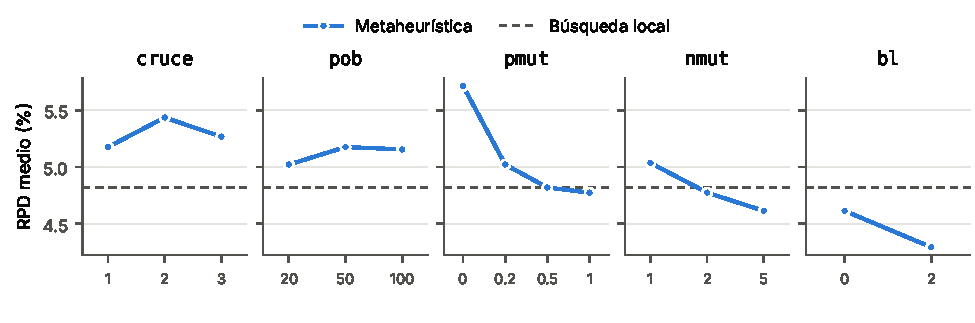
\includegraphics[width=\textwidth]{figuras/cal_genetico.pdf}
\caption{Algoritmo Genético: RPD medio según el valor de cada parámetro.}
\end{figure}

\begin{itemize}
  \item \textbf{\cod{cruce}.} El de un punto (5.18) es mejor que el ponderado (5.27) y que
        el uniforme (5.44). El cruce de un punto conserva juntos bloques enteros de columnas
        de cada progenitor, y con ellos trozos de solución que ya ``encajaban''; el uniforme
        los deshace gen a gen. Además es el más rápido (3\,400 generaciones frente a 2\,300).
  \item \textbf{\cod{pob}.} Población pequeña: 20 individuos (5.02) mejor que 50 o 100
        (5.18 y 5.16). Con el tiempo fijo, una población pequeña permite muchas más
        generaciones (12\,600 frente a 1\,100 con 100 individuos).
  \item \textbf{\cod{pmut}.} Aquí el resultado contradice la recomendación general de los
        apuntes (``probabilidad muy baja''): sin mutación el algoritmo es claramente peor
        (5.71) y mejora de forma continua hasta mutar \emph{todos} los hijos (4.77). La
        explicación es que la población es pequeña y, tras la reparación voraz, los hijos
        se parecen mucho a los padres: sin mutación la diversidad se agota enseguida. En
        este diseño la mutación (quitar columnas y reparar) hace el papel de la perturbación
        del temple y de la VNS, y es el verdadero motor de la búsqueda.
  \item \textbf{\cod{nmut}.} En la misma línea: mejor alterar 5 genes (4.61) que 1 o 2. Gana
        el extremo de la lista, así que es otro candidato para la segunda vuelta.
  \item \textbf{\cod{bl}.} Aplicar búsqueda local a los hijos (versión memética) mejora de
        4.61 a 4.29 aunque el número de generaciones se reduce a la tercera parte. Solo se
        ha probado con dos entornos; a la vista de lo que aporta $\D3$ en GRASP y VNS,
        \cod{bl}~$=3$ es el valor que la segunda vuelta opcional añade a la lista.
\end{itemize}

\textbf{Configuración elegida:} cruce de un punto, \cod{pob}~$=20$, \cod{pmut}~$=1$,
\cod{nmut}~$=5$, \cod{bl}~$=2$. El RPD pasa de 5.44 a 4.29: es el algoritmo que más gana con
la calibración, y también el que partía de la peor configuración base.

% ----------------------------------------------------------------------------
\subsection{Búsqueda en Entorno Variable}\label{sec:cal-vns}

\begin{table}[H]
\centering
\caption{Calibración de VNS. Cada fila es una etapa: RPD medio (\%) sobre las 18 ejecuciones (6 instancias $\times$ 3 semillas) de cada valor probado, con los demás parámetros fijos. En negrita, el mejor.}
\label{tab:cal-vns}
\small
\begin{tabular}{@{}cl>{\raggedright\arraybackslash}p{10.4cm}c@{}}
\toprule
Etapa & Parámetro & Valor probado $\rightarrow$ RPD medio & Elegido \\ \midrule
1 & \texttt{ja} & 1\,$\rightarrow$\,4.185;\quad 2\,$\rightarrow$\,4.228;\quad 3\,$\rightarrow$\,\textbf{3.625} & 3 \\
2 & \texttt{jb} & 2\,$\rightarrow$\,3.847;\quad 5\,$\rightarrow$\,3.625;\quad 10\,$\rightarrow$\,\textbf{3.625};\quad 20\,$\rightarrow$\,3.788 & 10 \\
3 & \texttt{lrc} & 1\,$\rightarrow$\,3.598;\quad 2\,$\rightarrow$\,3.625;\quad 3\,$\rightarrow$\,\textbf{3.585};\quad 5\,$\rightarrow$\,3.626 & 3 \\
\bottomrule
\end{tabular}
\end{table}

\begin{figure}[H]\centering
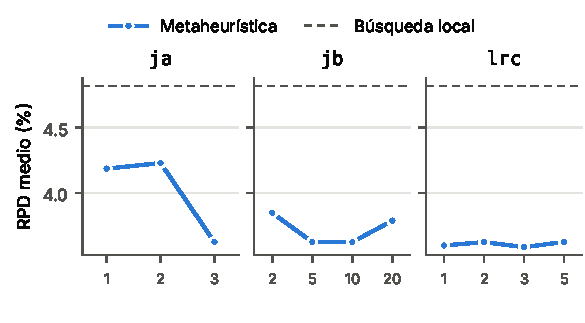
\includegraphics[width=0.68\textwidth]{figuras/cal_vns.pdf}
\caption{VNS: RPD medio según el valor de cada parámetro.}
\end{figure}

\begin{itemize}
  \item \textbf{\cod{ja} (entornos de la VND): parámetro crítico.} Con uno o dos entornos el
        RPD es 4.19 y 4.23; con los tres, 3.63, a pesar de que cada iteración es unas cien
        veces más cara (1\,700 iteraciones frente a 165\,000). Es la misma conclusión que en
        GRASP: el entorno $\D3$ es imprescindible.
  \item \textbf{\cod{jb} (tamaño máximo del salto).} Curva en U muy plana: 5 y 10 empatan
        (3.63; la media de 10 es menor por diezmilésimas, cualquiera de los dos vale), con 2
        los saltos son demasiado cortos para salir del óptimo local (3.85) y con 20
        demasiado largos (3.79).
  \item \textbf{\cod{lrc}.} Sin efecto apreciable: los cuatro valores quedan entre 3.59 y
        3.63, dentro del ruido. Se toma el de menor media.
\end{itemize}

\textbf{Configuración elegida:} $j_A=3$, $j_B=10$, \cod{lrc}~$=3$. El RPD pasa de 3.63 a
3.59: la configuración base ya era prácticamente la mejor. La VNS es, junto con la búsqueda
tabú, la metaheurística más robusta frente a sus parámetros, con la ventaja de que solo
tiene tres.

% ----------------------------------------------------------------------------
\subsection{Resumen de la calibración}

\begin{table}[H]
\centering
\caption{Configuración de partida (base) y configuración final de cada metaheurística, con su RPD medio (\%) en las instancias de calibración. En negrita, los valores que la calibración ha cambiado.}
\label{tab:config}
\begin{tabular}{@{}llcc@{}}
\toprule
Algoritmo & Parámetro & Base & Final \\ \midrule
Temple Simulado & \texttt{k} & 2 & 2 \\
 & \texttt{lrc} & 2 & 2 \\
 & \texttt{p0} & 0.5 & \textbf{0.1} \\
 & \texttt{alfa} & 0.95 & \textbf{0.99} \\
 & \texttt{L} & 1000 & 1000 \\
 & \emph{RPD medio} & \emph{4.597} & \emph{4.127} \\
\midrule
Búsqueda Tabú & \texttt{tent} & 10 & \textbf{20} \\
 & \texttt{tsal} & 3 & \textbf{1} \\
 & \texttt{beta} & 0.01 & 0.01 \\
 & \texttt{reinicio} & 2000 & \textbf{$10^6$} \\
 & \emph{RPD medio} & \emph{4.136} & \emph{4.095} \\
\midrule
GRASP & \texttt{lrc} & 3 & \textbf{10} \\
 & \texttt{lamf} & 0.5 & \textbf{0.2} \\
 & \texttt{elite} & 10 & \textbf{5} \\
 & \texttt{grent} & 3 & 3 \\
 & \emph{RPD medio} & \emph{3.952} & \emph{3.441} \\
\midrule
Algoritmo Genético & \texttt{cruce} & 2 & \textbf{1} \\
 & \texttt{pob} & 50 & \textbf{20} \\
 & \texttt{pmut} & 0.2 & \textbf{1.0} \\
 & \texttt{nmut} & 2 & \textbf{5} \\
 & \texttt{bl} & 0 & \textbf{2} \\
 & \emph{RPD medio} & \emph{5.436} & \emph{4.292} \\
\midrule
VNS & \texttt{ja} & 3 & 3 \\
 & \texttt{jb} & 5 & \textbf{10} \\
 & \texttt{lrc} & 2 & \textbf{3} \\
 & \emph{RPD medio} & \emph{3.625} & \emph{3.585} \\
\bottomrule
\end{tabular}
\end{table}


Lecciones generales de la calibración:
\begin{enumerate}
  \item \textbf{El entorno $\D3$ es el ingrediente decisivo.} Los algoritmos que lo usan en
        su búsqueda local (GRASP y VNS) son los mejores, y en ambos quitarlo cuesta entre
        seis décimas y un punto.
  \item \textbf{Los parámetros que más importan son los que fijan el tamaño del paso}
        ($k$ en el temple) \textbf{y el reparto del tiempo} ($\alpha$ y $L$ en el temple,
        el tamaño de la población en el genético). Un valor malo de estos parámetros anula
        el algoritmo: el temple con $k=1$ o con $L=5000$ no mejora al constructivo.
  \item \textbf{Los mecanismos de memoria dan resultados dispares}: la memoria de GRASP es
        muy valiosa; la penalización por frecuencia y la intensificación de la búsqueda tabú,
        casi irrelevantes.
  \item \textbf{Todas las metaheurísticas calibradas mejoran a la búsqueda local} (4.82),
        pero ninguna baja del 3.4\,\%. La sección~\ref{sec:conclusiones} analiza por qué.
\end{enumerate}
